\documentclass{my-article}
\usepackage{my-coverpage}
\usepackage{my-codespace}

\usepackage[utf8]{inputenc}
\usepackage[T5]{fontenc}
\usepackage[vietnamese]{babel}

\NameUpperUniname{Vietnam National University Ho Chi Minh City}
\NameUniname{Ho Chi Minh City University of Technology}
\NameDeptname{Faculty of Electrical and Electronics Engineering}
\NamePathlogo{./my-chapters/my-images/01_logobachkhoatoi.png}
\NamePathBackground[width=\paperwidth,height=\paperheight]{./my-chapters/my-images/bia.jpg} 
\NameGroup{}
\NameClass{}
\NameLesson[\Large]{PROJECT2 REPORT}
\NameTitle[\Large]{Sorting base-on FPGA}
\NameStudent{Nguyễn Đại Đồng}
\NameIDStudent{2210780}
\NameAdvisor{Nguyễn Trung Hiếu}
\NamePlace{Ho Chi Minh}
\NameTime{../../20..}


\begin{document}

\MycoverProject
\newpage
\fontsize{13}{14}\selectfont
\pagestyle{fancy}
\MycountPages{roman}
\tableofcontents
\listoffigures
\listoftables
\listoflistings
\newpage
\MychapterAbstract{
	Đồ án thực hiện một bộ có thể cho phép phần cứng sắp xếp dữ liệu trên một mảng lớn (tầm GB) mà không cần sử dụng đến CPU, giúp giải quyết được vấn đề liên quan việc tổn hao trên bus khi sử dụng CPU giao tiếp với Memory External.
}
\newpage
\MychapterAcknowledgement{
	Xin cảm ơn thầy Nguyễn Trung Hiếu.
}
\newpage
\fancyhead[R]{Advisor: {\fontencoding{T5}\selectfont Nguyễn Trung Hiếu}}
\MycountPages{number}
\section{Introduction}

\subsection{Đặt vấn đề}

Trong kỷ nguyên số hóa hiện nay, sự bùng nổ của Dữ liệu lớn (Big Data), Internet of Think (IoT) và Trí tuệ nhân tạo (AI) đã dẫn đến sự gia tăng theo cấp số nhân về khối lượng dữ liệu cần lưu trữ và xử lý. Sắp xếp dữ liệu (Data Sorting) không chỉ đơn thuần là việc tổ chức lại thông tin mà còn là một kernel tính toán nền tảng (fundamental computational kernel) quyết định hiệu năng của toàn bộ hệ thống. Sắp xếp đóng vai trò tiền đề thiết yếu cho các thuật toán tìm kiếm (như Binary Search), nén dữ liệu, loại bỏ trùng lặp và tối ưu hóa truy vấn cơ sở dữ liệu.

Các lĩnh vực yêu cầu lưu trữ và xử lý lượng dữ liệu khổng lồ bao gồm:
\begin{itemize}[label=-]
	\item Hệ quản trị cơ sở dữ liệu (Database Management Systems): Sắp xếp là bước bắt buộc để tạo chỉ mục (indexing), giúp tăng tốc độ truy vấn SQL và tối ưu hóa các phép toán JOIN.
	
	\item Trí tuệ nhân tạo và Học máy (AI/ML): Các thuật toán như k-Nearest Neighbors (k-NN), lọc trung vị (median filtering) trong xử lý ảnh, và tiền xử lý dữ liệu huấn luyện đều phụ thuộc nặng nề vào tốc độ sắp xếp.
	
	\item Viễn thông và Mạng (5G/6G \& IoT): Trong các hệ thống MIMO quy mô lớn hoặc định tuyến gói tin, việc sắp xếp dữ liệu tín hiệu và ưu tiên luồng dữ liệu (traffic shaping) đòi hỏi độ trễ cực thấp.
	
	\item Tin sinh học (Bioinformatics): Sắp xếp các chuỗi gen và protein để tìm kiếm mẫu tương đồng trong các cơ sở dữ liệu sinh học khổng lồ.
\end{itemize}

\subsection{Thách thức trong thiết kế phần cứng}

\subsubsection{Thách thức của Kiến trúc Máy tính Truyền thống và Hạn chế của Thuật toán Hiện hành}

\begin{enumerate}[label=\alph*.]
	\item Giới hạn của Kiến trúc Von Neumann và Bức tường Bộ nhớ
	
	Trong bối cảnh bùng nổ của các ứng dụng thâm dụng dữ liệu (Data-intensive applications) như Big Data và IoT, kiến trúc máy tính truyền thống Von Neumann đang đối mặt với những giới hạn vật lý nghiêm trọng. Sự chênh lệch ngày càng lớn giữa tốc độ xử lý của CPU và tốc độ truy xuất bộ nhớ đã tạo ra hiện tượng \textit{"Bức tường bộ nhớ"} (Memory Wall). Việc di chuyển khối lượng lớn dữ liệu chưa được sắp xếp giữa bộ nhớ ngoại vi (Off-chip DRAM) và bộ vi xử lý trung tâm (Host CPU) thông qua Bus hệ thống dẫn đến hai vấn đề cốt lõi trong thiết kế vi mạch:
	\begin{itemize}
		\item \textbf{Độ trễ truy xuất (Access Latency):} Thời gian chờ dữ liệu từ DRAM làm giảm hiệu suất thực thi của pipeline xử lý.
		\item \textbf{Tiêu thụ năng lượng động (Dynamic Power Consumption):} Việc chuyển đổi trạng thái liên tục trên Bus dữ liệu gây hao phí năng lượng đáng kể, đi ngược lại các tiêu chuẩn về thiết kế công suất thấp (Low-power design).
	\end{itemize}
	
	\item Hạn chế của Thuật toán Sắp xếp Kinh điển trong Triển khai Phần cứng
	
	Mặc dù các thuật toán như Merge-sort và Quick-sort hoạt động hiệu quả trên phần mềm, việc ánh xạ chúng lên kiến trúc phần cứng song song (Parallel Hardware Architecture) gặp nhiều trở ngại:
	\begin{itemize}
		\item \textbf{Merge-sort:} Tồn tại tính chất tuần tự cao trong giai đoạn hợp nhất (Merge phase), tạo ra các phụ thuộc dữ liệu (Data dependency) khiến việc thiết kế các bộ xử lý song song hoàn toàn trở nên bất khả thi mà không tiêu tốn tài nguyên bộ nhớ đệm (Buffer memory) lớn.
		\item \textbf{Quick-sort:} Việc lựa chọn phần tử chốt (Pivot) ngẫu nhiên thường dẫn đến việc phân hoạch không đồng đều, tạo ra các mảng con mất cân bằng (Unbalanced subarrays). Trong phần cứng, điều này gây ra hiện tượng \textit{mất cân bằng tải} (Load Imbalance) giữa các đơn vị xử lý (Processing Units - PUs), khiến một số lõi hoàn thành sớm và rơi vào trạng thái rỗi (Idle state), làm giảm hiệu suất sử dụng tài nguyên (Resource Utilization).
	\end{itemize}
\end{enumerate}

\subsubsection{Đề xuất Giải pháp Kiến trúc Processing-In-Memory (PIM)}

\begin{enumerate}[label=\alph*.]
	\item Chuyển dịch sang Xử lý Tại Bộ nhớ (Near-Memory Processing)
	
	Để giải quyết nút thắt cổ chai về băng thông và độ trễ, đồ án đề xuất thiết kế một lõi IP (Intellectual Property Core) hoạt động theo cơ chế \textit{Processing-In-Memory} (PIM). Kiến trúc này cho phép thực thi tác vụ sắp xếp ngay tại miền bộ nhớ, giảm tải (Offload) hoàn toàn cho Host CPU và giảm thiểu lưu lượng giao tiếp trên Bus (Bus Traffic Reduction).
	
	\item Kỹ thuật Phân hoạch Dựa trên Giá trị Trung bình (Mean-based Partitioning)
	
	Thiết kế phần cứng đề xuất áp dụng phương pháp phân hoạch dữ liệu dựa trên giá trị trung bình để chia tập dữ liệu lớn thành các mảng con độc lập có kích thước xấp xỉ bằng nhau (Independent subarrays of approximately equal length). Phương pháp này mang lại các ưu điểm vượt trội cho thiết kế IC:
	\begin{itemize}
		\item \textbf{Cân bằng tải (Load Balancing):} Đảm bảo khối lượng tính toán được phân phối đều giữa các lõi xử lý song song, tối đa hóa thông lượng (Throughput).
		\item \textbf{Kiến trúc Tự chủ (CPU-less Architecture):} Các mảng con độc lập cho phép các khối phần cứng hoạt động song song mà không cần cơ chế đồng bộ hóa phức tạp hay sự điều phối từ CPU.
		\item \textbf{Tối ưu hóa Năng lượng (Energy Efficiency):} Việc thực hiện sắp xếp tại chỗ (In-place sorting) và loại bỏ các thao tác I/O dư thừa giúp cải thiện đáng kể chỉ số hiệu năng trên mỗi watt (Performance-per-Watt).
	\end{itemize}
\end{enumerate}

\subsection{Mục tiêu của báo cáo}

Mục tiêu của đồ án là thiết kế một kiến trúc \textbf{Processing-In-Memory (PIM)} đóng vai trò như một bộ tăng tốc phần cứng (Hardware Accelerator), cho phép sắp xếp các tập dữ liệu kích thước lớn lưu trữ tại bộ nhớ ngoài (Off-chip Memory/DRAM) mà giảm thiểu tối đa sự phụ thuộc vào vi xử lý trung tâm (Host CPU).

Khối thiết kế này ứng dụng kỹ thuật phân hoạch dữ liệu thành các mảng con độc lập (Independent Subarrays) và thực hiện sắp xếp tại chỗ (In-place). Cơ chế này giúp loại bỏ nhu cầu di chuyển dữ liệu liên tục qua Bus hệ thống, từ đó giải quyết triệt để vấn đề nút thắt băng thông (Memory Wall) và tiêu hao năng lượng do truyền tải dữ liệu. Bằng cách giảm tải (offload) tác vụ sắp xếp khỏi CPU, thiết kế giúp tối ưu hóa hiệu năng tổng thể và hiệu quả năng lượng cho các ứng dụng xử lý dữ liệu lớn (Big Data applications).
\section{Literature Review}

Nghiên cứu này được xây dựng dựa trên nền tảng lý thuyết của framework sắp xếp dữ liệu đề xuất bởi Shahriar Shirvani Moghaddam và Kiaksar Shirvani Moghaddam trong công trình \textit{"A General Framework for Sorting Large Data Sets Using Independent Subarrays of Approximately Equal Length"}\cite{moghaddam2022general}. Khác với các phương pháp tiếp cận truyền thống thường tập trung vào việc tối ưu hóa một thuật toán cụ thể, framework này cung cấp một cơ chế tổng quát để chia nhỏ bài toán sắp xếp lớn thành các tác vụ độc lập, tạo tiền đề cho việc xử lý song song hiệu quả.

Cơ chế hoạt động của framework được chia thành ba giai đoạn chính (phases), được thiết kế để khắc phục nhược điểm mất cân bằng tải thường thấy ở Quick-sort truyền thống:

\begin{enumerate}[label=\textbf{Phase \arabic*.}, leftmargin=2cm]
	\item Sorted/Similar Checker - SS Checker
	
	Trước khi thực hiện bất kỳ thao tác phân hoạch nào, framework thực hiện một bước kiểm tra trạng thái dữ liệu đầu vào. Khối \textit{SS Checker} có nhiệm vụ xác định xem mảng dữ liệu hiện tại có thuộc một trong các trường hợp đặc biệt sau hay không:
	\begin{itemize}
		\item Đã được sắp xếp hoàn toàn (Sorted).
		\item Được sắp xếp theo thứ tự ngược (Reversely sorted).
		\item Chứa các phần tử giống hệt nhau (Similar elements).
	\end{itemize}
	Việc phát hiện sớm các trường hợp này giúp hệ thống bỏ qua các bước tính toán dư thừa, từ đó giảm thiểu độ phức tạp thời gian trong các trường hợp tốt nhất (Best-case scenario).
	
	\item Mean-based Partitioning
		
	Đây là giai đoạn cốt lõi tạo nên tính ưu việt của giải thuật đối với thiết kế phần cứng. Thay vì chọn phần tử chốt (pivot) ngẫu nhiên như Quick-sort, framework tính toán giá trị trung bình (Mean value) của toàn bộ mảng dữ liệu.
	\begin{itemize}
		\item Dữ liệu được so sánh với giá trị Mean và chia thành hai mảng con: một mảng chứa các giá trị nhỏ hơn Mean và mảng còn lại chứa các giá trị lớn hơn hoặc bằng Mean.
		\item Quá trình này được thực hiện đệ quy qua $M$ cấp độ (Levels), tạo ra $2^M$ mảng con.
		\item \textbf{Đặc tính quan trọng:} Các tác giả đã chứng minh rằng việc sử dụng Mean làm pivot giúp tạo ra các mảng con có độ dài xấp xỉ bằng nhau (Approximately equal length) ngay cả với các phân phối dữ liệu bất đối xứng. Điều này đảm bảo tính cân bằng tải (Load balancing) tuyệt đối khi ánh xạ lên các phần tử xử lý song song.
	\end{itemize}
	
	\item Core-Sort
	
	Sau khi đạt đến số lượng phân hoạch $M$ định trước, các mảng con độc lập (Independent Subarrays) sẽ được sắp xếp riêng biệt bằng một thuật toán lõi (Core-sort) như Quick-sort hoặc Merge-sort. 
	
	Do các mảng con đã được phân tách hoàn toàn về mặt giá trị (mọi phần tử ở mảng con $i$ đều nhỏ hơn mảng con $i+1$), quá trình này có thể thực hiện song song hoàn toàn trên các lõi xử lý phần cứng mà không cần cơ chế đồng bộ hóa hay trao đổi dữ liệu giữa các luồng (Inter-processor communication).
	
	Tổng hợp lại, framework này cung cấp một kiến trúc lý tưởng cho thiết kế \textit{Processing-In-Memory} (PIM) hướng tới mục tiêu CPU-less, vì nó loại bỏ sự phụ thuộc dữ liệu và cho phép các khối logic tính toán hoạt động định hình và cô lập.
\end{enumerate}

\subsection{Thực hiện lại Framework của bài báo}

Trong bài báo nêu ra được cải thiện độ phức tạp khi sử dụng framework trong việc sử dụng thuật toán QuickSort và MergeSort như sau:

\begin{table}[H]
	\renewcommand{\arraystretch}{2.2}
	\fontsize{11}{13}\selectfont
	\caption{The time complexity of the conventional and proposed Quick and Merge sorts in the best, average, and worst cases.} 
	\label{tab:complexity}
	\hspace*{-1.5cm}%
	\begin{tabular}{|>{\centering\arraybackslash}m{1.5cm}
			|>{\centering\arraybackslash}m{2.5cm}
			|>{\centering\arraybackslash}m{4.5cm}
			|>{\centering\arraybackslash}m{4.5cm}
			|>{\centering\arraybackslash}m{4.5cm}|}
		
		\hline
		\textbf{} & \textbf{Method} & \textbf{Best-case} & \textbf{Average-case} & \textbf{Worst-case} \\
		\hline
		
		% --- QUICK SORT SECTION ---
%		\multirow{6}{*}{\textbf{Quick}} 
		& Conventional & $O(N \log N)$ & $O(N \log N)$ & $O(N^2)$ \\ \cline{2-5}
		
		\textbf{Quick} & Proposed serial & $\begin{cases} O(2N), & \text{ord./sim.} \\ O(3N), & \text{rev. ord.} \end{cases}$ & $O(4M.N) + O(N \log(\frac{N}{2^M}))$ & $O(4M.N) + O((2^M - k)\frac{N}{2^M} \log(\frac{N}{2^M}) + k\frac{N^2}{2^{2M}})$ \\ \cline{2-5}       
		
		& Proposed parallel & $\begin{cases} O(\frac{2N}{2^M} + 2M), & \text{ord./sim.} \\ O(\frac{3N}{2^M} + 3M), & \text{rev. ord.} \end{cases}$ & $O(4M(\frac{N}{2^M} + 2^M - 1)) + O(\frac{N}{2^M} \log(\frac{N}{2^M}))$ & $O(4M(\frac{N}{2^M} + 2^M - 1)) + O(\frac{N^2}{2^{2M}})$ \\ \hline
		
		% --- MERGE SORT SECTION ---
%		\multirow{6}{*}{\textbf{Merge}} 
		& Conventional & $O(N \log N)$ & $O(N \log N)$ & $O(N \log N)$ \\ \cline{2-5}
		
		\textbf{Merge} & Proposed serial 
		& $\begin{cases} O(2N), & \text{ord./sim.} \\ O(3N), & \text{rev. ord.} \end{cases}$ 
		& $O(4M.N) + O(N \log(\frac{N}{2^M}))$ 
		& $O(4M.N) + O(N \log(\frac{N}{2^M}))$ \\ \cline{2-5}
		
		& Proposed parallel 
		& $\begin{cases} O(\frac{2N}{2^M} + 2M), & \text{ord./sim.} \\ O(\frac{3N}{2^M} + 3M), & \text{rev. ord.} \end{cases}$ 
		& $O(4M(\frac{N}{2^M} + 2^M - 1)) + O(\frac{N}{2^M} \log(\frac{N}{2^M}))$ 
		& $O(4M(\frac{N}{2^M} + 2^M - 1)) + O(\frac{N}{2^M} \log(\frac{N}{2^M}))$ \\
		\hline
	\end{tabular}
\end{table}

Và đây là đoạn code pseudo thực hiện:

\lstinputlisting[
basicstyle=\fontsize{10}{11}\selectfont\ttfamily,
style=StylePseudo,
language=Pseudo,
caption={The Pseudo-Code of the Serial Realization of the Proposed Mean-Based Data Sorting Framework.},
label=pseudo-code:Serial
]{./my-chapters/my-codes/pseudo_serial.txt}

Ta tiến hành thực hiện việc so các giải thuật trên với các phần tử số thực như sau:

\begin{lstlisting}[style=StylePseudo, language=Pseudo]
	-1344457441.558848 1837028809.6233559 ... 1967142726.7494054 421697126.41092634
\end{lstlisting}

\begin{lstlisting}[style=StyleResult, language=Result, basicstyle=\fontsize{6}{6}\selectfont\ttfamily, caption={Kết quả kiểm chứng khi chạy với $N = 2^{17}$.}]
	Finished reading file: ./tools/unsorted.txt
	Finish write file './Reports/COMPILE_REPORT/unsorted.txt'.
	Size of array: 131072
	Number subarry M = 5
	[FrameworkStandard_Quick] Number of Similar = 0
	[FrameworkStandard_Quick] Number of Ascending = 83
	[FrameworkStandard_Quick] Number of Descending = 84
	[FrameworkStandard_Merge] Number of Similar = 0
	[FrameworkStandard_Merge] Number of Ascending = 83
	[FrameworkStandard_Merge] Number of Descending = 84
	
	Sort algorithm                Check sorted   Time (ns)           Number Swap         Number Compare      
	--------------------------------------------------------------------------------------------------------------
	Data Set                      FAIL           0                   0                   0                   
	--------------------------------------------------------------------------------------------------------------
	Sort Standard                 PASS           6776394             0                   0                   
	--------------------------------------------------------------------------------------------------------------
	QuickSort                     PASS           8550932             2664420             1422629             
	--------------------------------------------------------------------------------------------------------------
	Framework_QuickSort           PASS           10602239            128005830           63593393            
	--------------------------------------------------------------------------------------------------------------
	MergeSort                     PASS           8682661             2664420             1422629             
	--------------------------------------------------------------------------------------------------------------
	Framework_Merge               PASS           14602192            370425084           134830050           
	--------------------------------------------------------------------------------------------------------------
\end{lstlisting}

\begin{lstlisting}[style=StyleResult, language=Result, basicstyle=\fontsize{9}{10}\selectfont\ttfamily, caption={Kiểm tra sử dụng bộ nhớ khi sử dụng QuickSort.}]
	--------------------------------------------------------------------------------
	Command:            ./main 5 2
	Massif arguments:   --stacks=yes --massif-out-file=Reports/ANALYSIS_DIR/checkmemory/QuickSort_Result.out
	ms_print arguments: Reports/ANALYSIS_DIR/checkmemory/QuickSort_Result.out
	--------------------------------------------------------------------------------
	
	
	MB
	1.071^                                                                :::
	|                                                                    #:::
	|                                                                    #:::
	|                                                                    #:::
	|                                                                    #:::
	|             @                                                      #:::
	|             @                                                      #:::
	|             @                                                      #:::
	|             @                                                      #:::
	|             @                                                      #:::
	|             @::@:::@::@:::::::::::::::::::::@:::::@::::::@:::::@:::#:::
	|             @::@:::@::@:::::::::::::::::::::@:::::@::::::@:::::@:::#:::
	|             @::@:::@::@:::::::::::::::::::::@:::::@::::::@:::::@:::#:::
	|             @::@:::@::@:::::::::::::::::::::@:::::@::::::@:::::@:::#:::
	|       ::::::@::@:::@::@:::::::::::::::::::::@:::::@::::::@:::::@:::#:::
	|       ::::::@::@:::@::@:::::::::::::::::::::@:::::@::::::@:::::@:::#:::
	|       ::::::@::@:::@::@:::::::::::::::::::::@:::::@::::::@:::::@:::#:::
	|   ::::::::::@::@:::@::@:::::::::::::::::::::@:::::@::::::@:::::@:::#:::
	| ::: ::::::::@::@:::@::@:::::::::::::::::::::@:::::@::::::@:::::@:::#:::
	|:: : ::::::::@::@:::@::@:::::::::::::::::::::@:::::@::::::@:::::@:::#:::
	0 +----------------------------------------------------------------------->Mi
	0                                                                   787.9
	
	Number of snapshots: 96
	Detailed snapshots: [13, 17, 21, 25, 52, 62, 72, 82, 90 (peak)]
	
\end{lstlisting}

\begin{lstlisting}[style=StyleResult, language=Result, basicstyle=\fontsize{9}{10}\selectfont\ttfamily, caption={Kiểm tra sử dụng bộ nhớ khi sử dụng QuickSort kèm theo Framework.}]
	--------------------------------------------------------------------------------
	Command:            ./main 5 2
	Massif arguments:   --stacks=yes --massif-out-file=Reports/ANALYSIS_DIR/checkmemory/QuickSort_Convenlution_Result.out
	ms_print arguments: Reports/ANALYSIS_DIR/checkmemory/QuickSort_Convenlution_Result.out
	--------------------------------------------------------------------------------
	
	
	MB
	1.071^                                                                :  
	|                                                                    #:::
	|                                                                    #:::
	|                                                                    #:::
	|                                                                    #:::
	|             @                                                      #:::
	|             @                                                      #:::
	|             @                                                      #:::
	|             @                                                      #:::
	|             @                                                      #:::
	|             @:::::::::::::::@:@@:@:::::@:::::::::::::::::::@::::@::#:::
	|             @::: :::: ::::::@:@ :@:::: @: ::: :: :::: :::::@::::@::#:::
	|             @::: :::: ::::::@:@ :@:::: @: ::: :: :::: :::::@::::@::#:::
	|             @::: :::: ::::::@:@ :@:::: @: ::: :: :::: :::::@::::@::#:::
	|       ::::@:@::: :::: ::::::@:@ :@:::: @: ::: :: :::: :::::@::::@::#:::
	|       ::: @ @::: :::: ::::::@:@ :@:::: @: ::: :: :::: :::::@::::@::#:::
	|       ::: @ @::: :::: ::::::@:@ :@:::: @: ::: :: :::: :::::@::::@::#:::
	|   :@::::: @ @::: :::: ::::::@:@ :@:::: @: ::: :: :::: :::::@::::@::#:::
	| :::@::::: @ @::: :::: ::::::@:@ :@:::: @: ::: :: :::: :::::@::::@::#:::
	| :::@::::: @ @::: :::: ::::::@:@ :@:::: @: ::: :: :::: :::::@::::@::#:::
	0 +----------------------------------------------------------------------->Mi
	0                                                                   796.8
	
	Number of snapshots: 81
	Detailed snapshots: [5, 11, 13, 27, 30, 32, 38, 58, 68, 73 (peak)]
\end{lstlisting}

\begin{lstlisting}[style=StyleResult, language=Result, basicstyle=\fontsize{9}{10}\selectfont\ttfamily, caption={Kiểm tra sử dụng bộ nhớ khi sử dụng MergeSort.}]
	--------------------------------------------------------------------------------
	Command:            ./main 5 2
	Massif arguments:   --stacks=yes --massif-out-file=Reports/ANALYSIS_DIR/checkmemory/MergeSort_Result.out
	ms_print arguments: Reports/ANALYSIS_DIR/checkmemory/MergeSort_Result.out
	--------------------------------------------------------------------------------
	
	
	MB
	1.071^                                                                :::
	|                                                                    #:::
	|                                                                    #:::
	|                                                                    #:::
	|                                                                    #:::
	|             @                                                      #:::
	|             @                                                      #:::
	|             @                                                      #:::
	|             @                                                      #:::
	|             @                                                      #:::
	|             @::@:::@::@:::::::::::::::::::::@:::::@::::::@:::::@:::#:::
	|             @::@:::@::@:::::::::::::::::::::@:::::@::::::@:::::@:::#:::
	|             @::@:::@::@:::::::::::::::::::::@:::::@::::::@:::::@:::#:::
	|             @::@:::@::@:::::::::::::::::::::@:::::@::::::@:::::@:::#:::
	|       ::::::@::@:::@::@:::::::::::::::::::::@:::::@::::::@:::::@:::#:::
	|       ::::::@::@:::@::@:::::::::::::::::::::@:::::@::::::@:::::@:::#:::
	|       ::::::@::@:::@::@:::::::::::::::::::::@:::::@::::::@:::::@:::#:::
	|   ::::::::::@::@:::@::@:::::::::::::::::::::@:::::@::::::@:::::@:::#:::
	| ::: ::::::::@::@:::@::@:::::::::::::::::::::@:::::@::::::@:::::@:::#:::
	|:: : ::::::::@::@:::@::@:::::::::::::::::::::@:::::@::::::@:::::@:::#:::
	0 +----------------------------------------------------------------------->Mi
	0                                                                   787.9
	
	Number of snapshots: 96
	Detailed snapshots: [13, 17, 21, 25, 52, 62, 72, 82, 90 (peak)]
\end{lstlisting}

\begin{lstlisting}[style=StyleResult, language=Result, basicstyle=\fontsize{9}{10}\selectfont\ttfamily, caption={Kiểm tra sử dụng bộ nhớ khi sử dụng MergeSort kèm theo Framework.}]
	--------------------------------------------------------------------------------
	Command:            ./main 5 2
	Massif arguments:   --stacks=yes --massif-out-file=Reports/ANALYSIS_DIR/checkmemory/MergeSort_Convulation_Result.out
	ms_print arguments: Reports/ANALYSIS_DIR/checkmemory/MergeSort_Convulation_Result.out
	--------------------------------------------------------------------------------
	
	
	MB
	1.134^                                                               #   
	|                                                                  @@#   
	|                                                                 @@@#:::
	|                                                                 @@@#:::
	|                                                                 @@@#:::
	|                                                                 @@@#:::
	|            @                                                    @@@#:::
	|            @                                                    @@@#:::
	|            @                                                    @@@#:::
	|            @                                                    @@@#:::
	|            @:::::::::::::::@:@@:@:::::@:::::::::::::::::@::::@::@@@#:::
	|            @::: ::: :::::: @:@ :@:: ::@:::: ::: ::: ::::@::::@::@@@#:::
	|            @::: ::: :::::: @:@ :@:: ::@:::: ::: ::: ::::@::::@::@@@#:::
	|            @::: ::: :::::: @:@ :@:: ::@:::: ::: ::: ::::@::::@::@@@#:::
	|            @::: ::: :::::: @:@ :@:: ::@:::: ::: ::: ::::@::::@::@@@#:::
	|       :::@:@::: ::: :::::: @:@ :@:: ::@:::: ::: ::: ::::@::::@::@@@#:::
	|       :::@:@::: ::: :::::: @:@ :@:: ::@:::: ::: ::: ::::@::::@::@@@#:::
	|   :@:::::@:@::: ::: :::::: @:@ :@:: ::@:::: ::: ::: ::::@::::@::@@@#:::
	| :::@:::::@:@::: ::: :::::: @:@ :@:: ::@:::: ::: ::: ::::@::::@::@@@#:::
	| :::@:::::@:@::: ::: :::::: @:@ :@:: ::@:::: ::: ::: ::::@::::@::@@@#:::
	0 +----------------------------------------------------------------------->Mi
	0                                                                   831.5
	
	Number of snapshots: 88
	Detailed snapshots: [5, 11, 13, 27, 30, 32, 38, 58, 68, 73, 76, 78, 81 (peak)]
\end{lstlisting}
\section{System Level Test}

Từ đoạn code mẫu \ref{pseudo-code:Serial} được nêu trong bài báo, có vài điểm cần phải phải tối ưu trong quá trình có thể chuyển từ giải thuật của bài báo xuông được phần cứng.

\subsection{Xây dựng Bộ tính giá trị trung bình của mảng}

\begin{lstlisting}[style=StyleCode, language=C, caption={Tính giá trị Trung bình.}]
	SIZE_TYPE_T C_Framework_RTL::P_Cal_Mean(std::vector<SIZE_ARR_T> &arr, IndexType si, IndexType ei){
		SIZE_TYPE_T t_sum = 0;
		for(int i =si; i <= ei; i++){
			t_sum += arr[i];
		}
		SIZE_TYPE_T t_div = 1;
		t_div = t_sum / (SIZE_TYPE_T)(ei - si + 1);
		return t_div;
	}
\end{lstlisting}

Với một bộ tính giá trị trung bình bằng cách đọc tất cả các giá trị trong mảng để tính được giá trị tổng quát của mảng. Còn giá trị số lượng phần tử được tính bằng công thức \texttt{(SIZE\_TYPE\_T)(ei - si + 1)} để chuyển từ giá trị HEX qua Float. Kết hợp thêm bộ kiểm tra các trường hợp đặc biệt của vùng dữ liệu:

%\begin{lstlisting}[style=StyleCode, language=C, caption={Tính giá trị Trung bình và Tìm trường hợp đặc biệt.}]
%	status_rtl_e C_Framework_RTL::P_SS_Check(std::vector<SIZE_ARR_T> &arr, IndexType si, IndexType ei, SIZE_TYPE_T &mean){
%		bool is_Similar     = true;
%		bool is_Acsending   = true;
%		bool is_Decsending  = true;
%		SIZE_TYPE_T temp_sum = 0;
%		for(int i = si + 1; i <= ei; ++i){
%			temp_sum += arr[i - 1];
%			if(arr[i] != arr[i - 1]){
%				is_Similar      = false;
%			}
%			if(arr[i] < arr[i - 1]){
%				is_Acsending    = false;
%			}
%			if(arr[i] > arr[i - 1]){
%				is_Decsending   = false;
%			}
%		}
%		temp_sum += arr[ei];
%		mean = temp_sum / (SIZE_TYPE_T)(ei - si + 1);
%		if(is_Similar){
%			return RTL_SIMILAR;
%		}
%		else if(is_Acsending){
%			return RTL_ACSENDING;
%		}
%		else if(is_Decsending){
%			return RTL_DESCENDING;
%		}
%		else{
%			return RTL_NORMAL;
%		}
%	};
%\end{lstlisting}
\begin{lstlisting}[style=StyleCode, language=C, caption={Tính giá trị Trung bình và Tìm trường hợp đặc biệt.}]
	status_rtl_e C_Framework_RTL::P_SS_Check(std::vector<SIZE_ARR_T> &arr, IndexType si, IndexType ei, SIZE_TYPE_T &mean){
		bool is_Similar     = true;
		bool is_Acsending   = true;
		bool is_Decsending  = true;
		SIZE_TYPE_T temp_sum = 0;
		for(int i = si; i < ei; ++i){
			temp_sum += arr[i];
			if(arr[i] != arr[i + 1]){
				is_Similar      = false;
			}
			if(arr[i] > arr[i + 1]){
				is_Acsending    = false;
			}
			if(arr[i] < arr[i + 1]){
				is_Decsending   = false;
			}
		}
		temp_sum += arr[ei];
		mean = temp_sum / (SIZE_TYPE_T)(ei - si + 1);
		if(is_Similar){
			return RTL_SIMILAR;
		}
		else if(is_Acsending){
			return RTL_ACSENDING;
		}
		else if(is_Decsending){
			return RTL_DESCENDING;
		}
		else{
			return RTL_NORMAL;
		}
	};
\end{lstlisting}

\subsection{Xây dựng bộ thực hiện phân hoạch mảng theo giá trị trung bình}

\begin{lstlisting}[style=StyleCode, language=C, caption={Phân hoạch dữ liệu theo giá trị trung bình.}]
	IndexType C_Framework_RTL::P_Partition_Iterative(std::vector<SIZE_ARR_T>& arr, IndexType si, IndexType ei, SIZE_TYPE_T mean_value) {
		IndexType pi = si;
		SIZE_ARR_T temp_a = 0;
		SIZE_ARR_T temp_pi = 0;
		for (IndexType i = si; i <= ei; ++i) {
			temp_a = arr[i];
			temp_pi = arr[pi];
			if (temp_a < mean_value) {
				arr[i] = temp_pi;
				arr[pi] = temp_a;
				pi++;
			}
		}
		return (pi > si) ? (pi - 1) : si; 
	}
\end{lstlisting}

Với việc tiến hành đọc dữ liệu trước khi so sánh dữ liệu với \texttt{pivot} giúp ta tối ưu và làm rõ được các bước làm trong phần cứng để có thể dễ dàng tiếp cận hơn. Với cách đó, chúng cho phép ta không cần sử dụng giải thuật \texttt{std::swap} để giúp giảm thiểu đơn vị swap.

\subsection{Xây dựng bộ thực hiện kiểm soát chia mảng dữ liệu}

\begin{lstlisting}[style=StyleCode, language=C, caption={Phân hoạch dữ liệu theo giá trị trung bình.}]
	void C_Framework_RTL::P_Division_Iterative(std::vector<SIZE_ARR_T>& arr, int M) {
		std::vector<PartitionTask> stack_registers;
		if (!arr.empty()) {
			stack_registers.push_back({0, static_cast<IndexType>(arr.size()) - 1, 0});
		}
		while (!stack_registers.empty()) {
			SIZE_TYPE_T mean_val = 0;
			PartitionTask task = stack_registers.back();
			stack_registers.pop_back();
			IndexType si = task.si;
			IndexType ei = task.ei;
			IndexType current_level = task.level;
			if (si >= ei) continue;
			RTL_state = P_SS_Check(arr, si, ei, mean_val);
			if (RTL_state == RTL_SIMILAR) {
				P_count_is_Sim++;
				continue; 
			}
			else if (RTL_state == RTL_ACSENDING) {
				P_count_is_Asc++;
				continue;
			}
			else if (RTL_state == RTL_DESCENDING) {
				P_count_is_Desc++;
				std::reverse(arr.begin() + si, arr.begin() + ei + 1);
				continue;
			} else {
				if (current_level < M) {
					IndexType bi = P_Partition_Iterative(arr, si, ei, mean_val);
					stack_registers.push_back({bi, ei, current_level + 1});
					stack_registers.push_back({si, bi, current_level + 1});
				} else {
					P_count_subarrays ++;
					F_QuickSort(arr, si, ei);
					P_count_compare += C_Sort_Algor::Get_Count_Compare();
					P_count_swap    += C_Sort_Algor::Get_Count_Swap();
				}
			}
		}
	}
\end{lstlisting}

Dựa trên việc kiểm soát luồng dữ liệu lưu hiện tại của mỗi đợt, ta sử dụng một stack lưu một dữ liệu hữu hạn của stack cho việc lưu trữ và kiểm soát các dữ liệu lưu giá trị \texttt{si} và \texttt{ei}.

\begin{figure}[H]
	\centering
	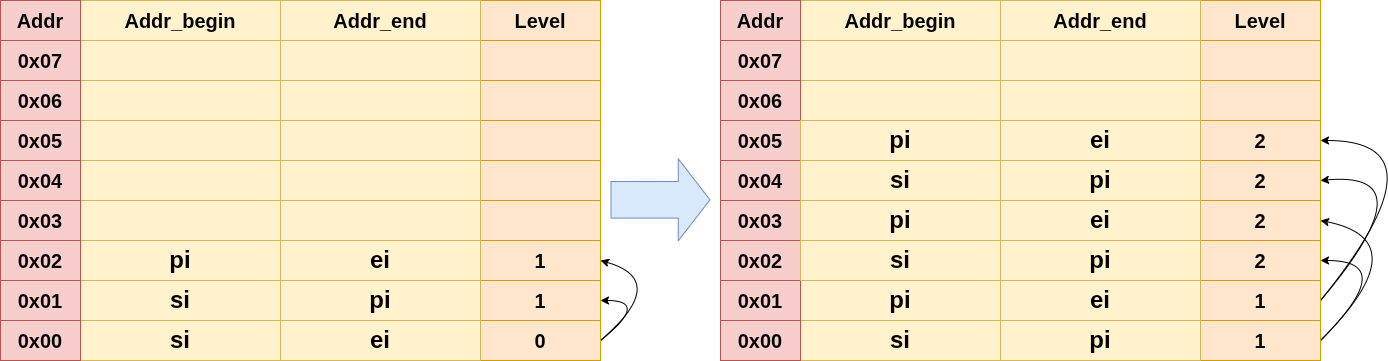
\includegraphics[width=.8\linewidth]{./my-chapters/my-images/SLT/stack_diagram.png}
	\caption{Cấu trúc của bộ lưu trữ stack khi thay thế cho đệ quy.}
\end{figure}

Nhờ đó, giải thuật đệ quy cho phép chia mảng thành từng đoạn $N/2$ được trực quan hóa hơn và dễ dàng kiểm soát hơn về mặt độ rộng, độ sâu của bộ nhớ stack thêm vào. Sau đây là so sánh giữa hai giải thuật:

\begin{table}[H]
	\centering
	{
		\fontsize{11}{10}\selectfont
		\renewcommand{\arraystretch}{1.5}
		\begin{tabular}{@{}p{4cm} p{5.5cm} p{5.5cm}@{}}
			\toprule
			\textbf{Tiêu chí} & \textbf{Recursive (Serial)} & \textbf{Iterative (RTL)} \\
			\midrule
			\textbf{Thời gian (Average Case)} & $O(N \log N)$ & $O(N \log N)$ \\
			\textbf{Thời gian (Worst Case)} & $O(N^2)$ & $O(N^2)$ \\
			\textbf{Không gian (Space)} & $O(M)$ hoặc $O(\log N)$ \newline (System Call Stack) & $O(M)$ hoặc $O(\log N)$ \newline (Heap Memory - \texttt{std::vector}) \\
			\textbf{Chi phí quản lý (Overhead)} & Cao (do khởi tạo stack frame cho mỗi lần gọi hàm). & Thấp (chỉ thao tác \texttt{push/pop} trên vector). \\
			\textbf{Rủi ro bộ nhớ} & Dễ gây \textit{Stack Overflow} khi $N$ lớn hoặc $M$ sâu. & An toàn hơn, giới hạn bởi dung lượng RAM (Heap). \\
			\bottomrule
		\end{tabular}
	}
	\caption{Bảng so sánh độ phức tạp và tài nguyên giữa bộ \texttt{Division\_Recursive} và bộ \texttt{Division\_Iterative}.}
\end{table}

\subsection{Kết quả của thuật toán sau khi viết lại}

\begin{figure}[H]
	\centering
	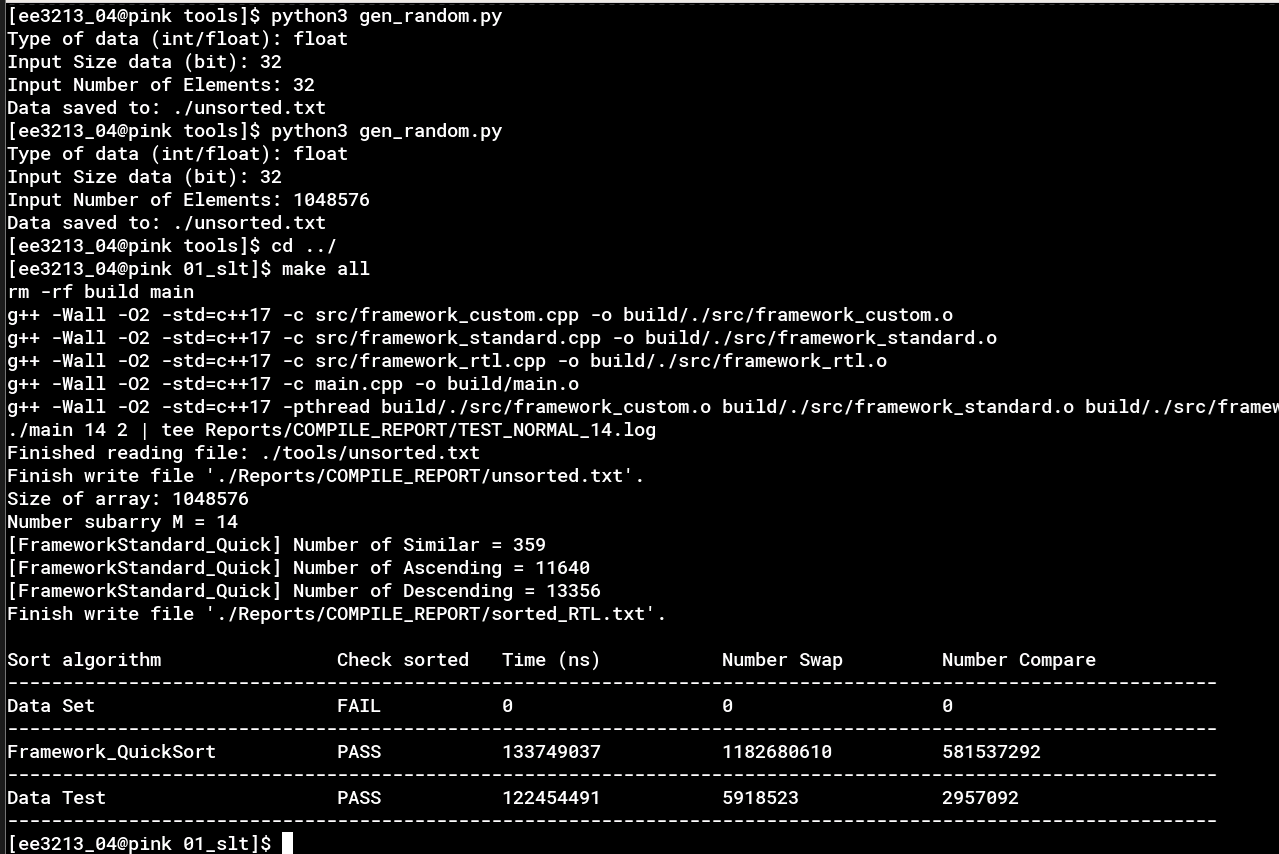
\includegraphics[width=.9\linewidth]{./my-chapters/my-images/SLT/Sort_2_20.png}
	\caption{Kết quả so sánh giữa bộ Framework chuẩn và Framework chỉnh sửa.}
\end{figure}

\begin{figure}[H]
	\centering
	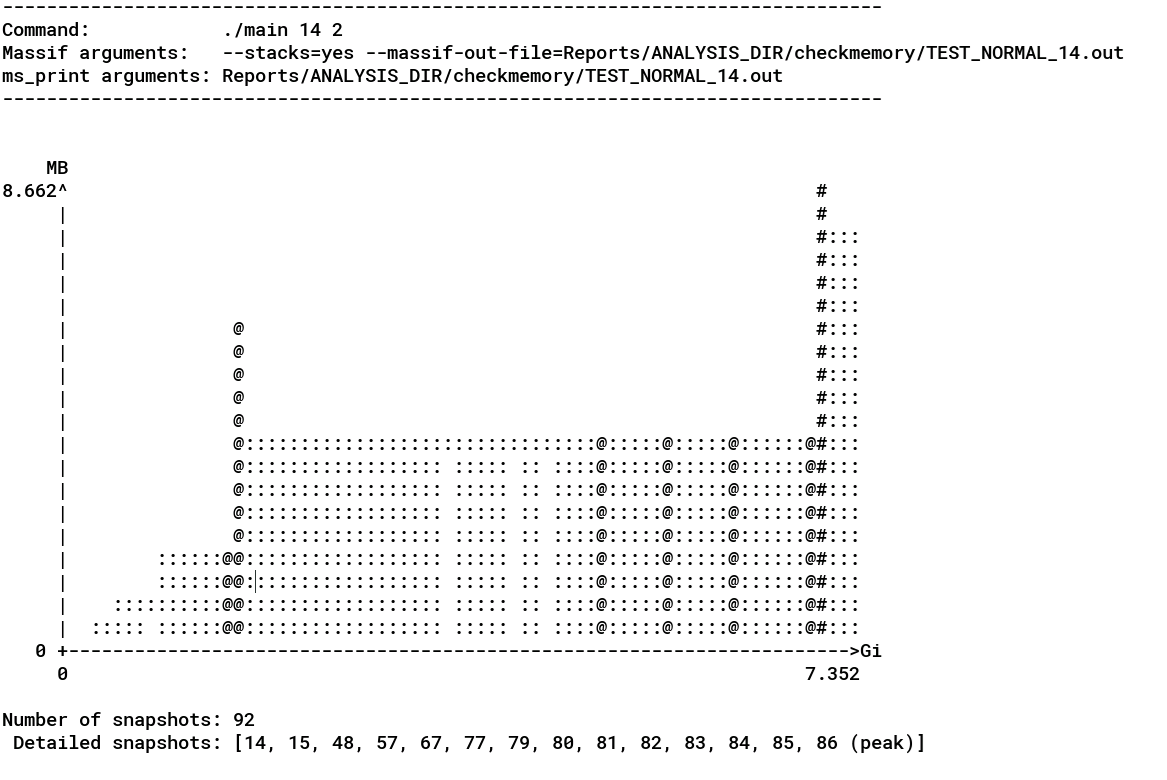
\includegraphics[width=.9\linewidth]{./my-chapters/my-images/SLT/mem_framework_standard_2_20.png}
	\caption{Kết quả của việc sử dụng Memory khi sử dụng Framework chuẩn.}
\end{figure}

\begin{figure}[H]
	\centering
	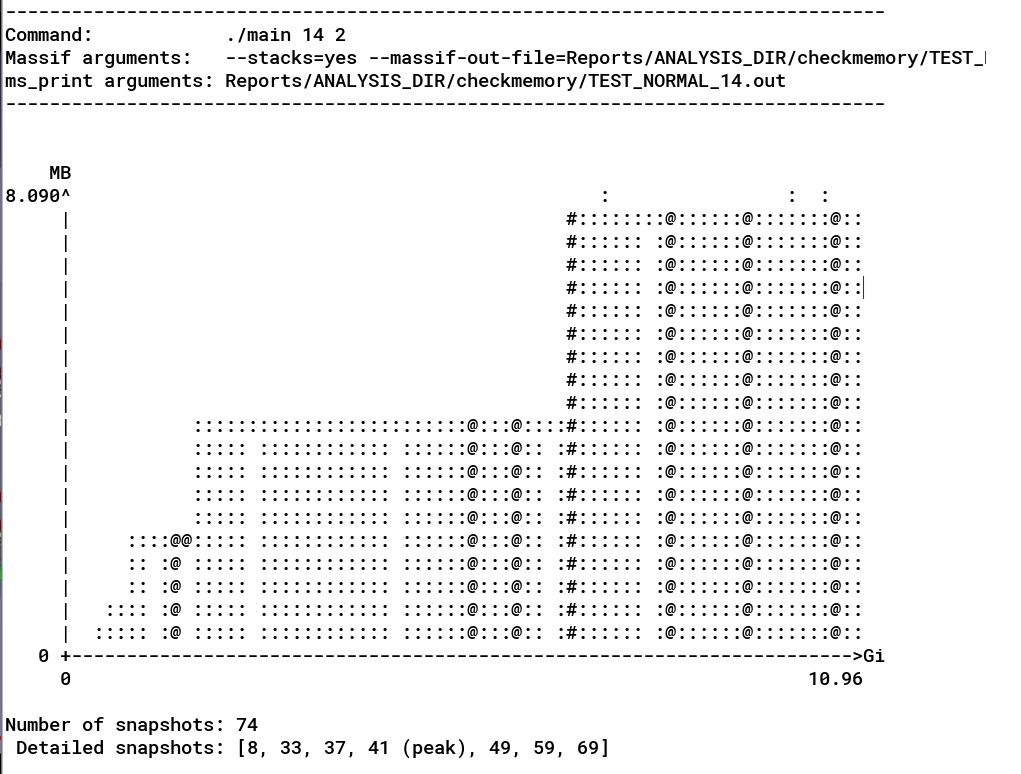
\includegraphics[width=.9\linewidth]{./my-chapters/my-images/SLT/mem_framework_rtl_2_20.png}
	\caption{Kết quả của việc sử dụng Memory khi sử dụng Framework chỉnh sửa.}
\end{figure}

Như vậy, sau khi tối ưu framework thì có số lượng Number Compare và Number Swap ít hơn tương đối so với framework chính thống.
\section{RTL Implementation}

\subsection{Bộ thực hiện tính giá trị trung bình của mảng (PACM\_UNIT)}

\subsubsection{Bộ tính cộng số thực (BFP16\_add)}

\begin{figure}[H]
	\centering
	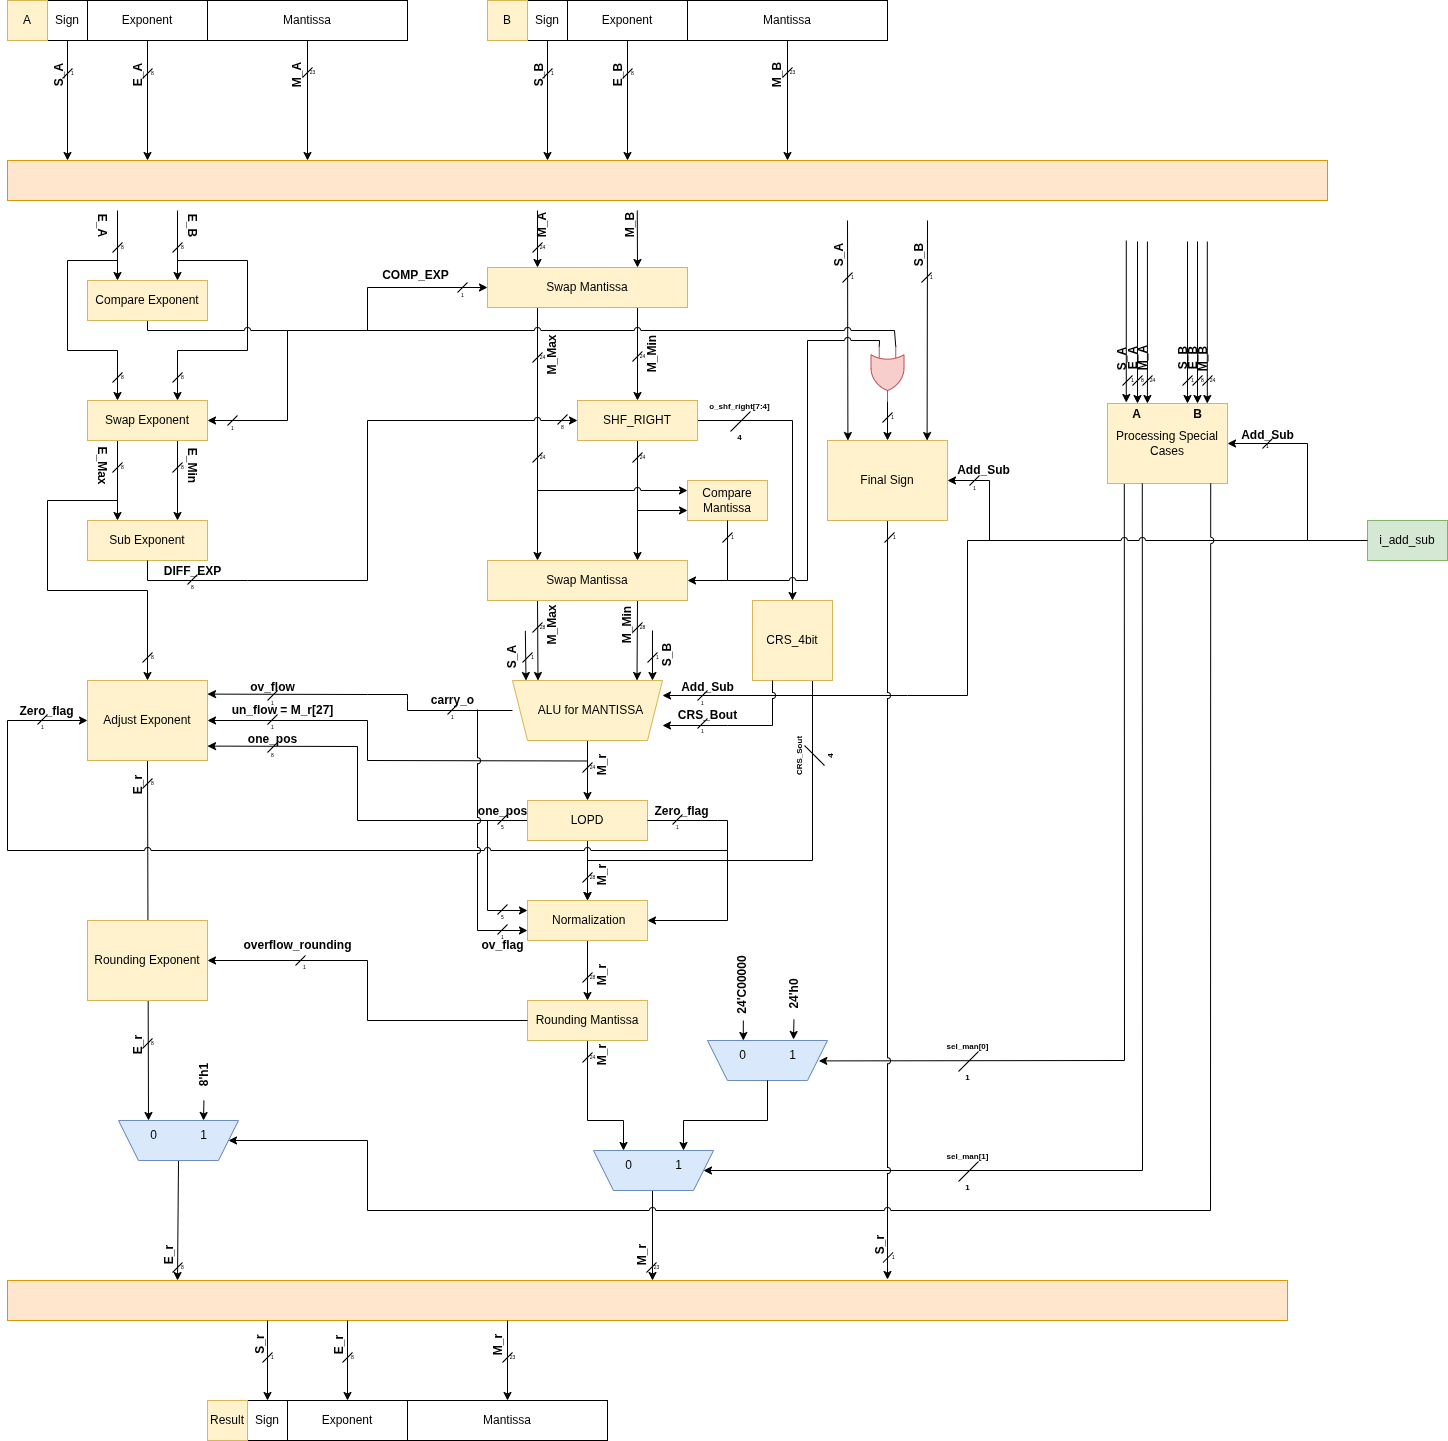
\includegraphics[width=.7\linewidth]{./../Version1/02_rtl/PA_CAL_MEAN/BFP16_ADD/00_spec/BlockDiagram_Overview.png}
	\caption{Bộ thực hiện 2 số Floating Point 32-bit.}
	\label{fig: RTL_BFP16}
\end{figure}



\subsubsection{Bộ tính cộng tích lũy của mảng (PA\_Cal\_Sum)}

\begin{figure}[H]
	\centering
	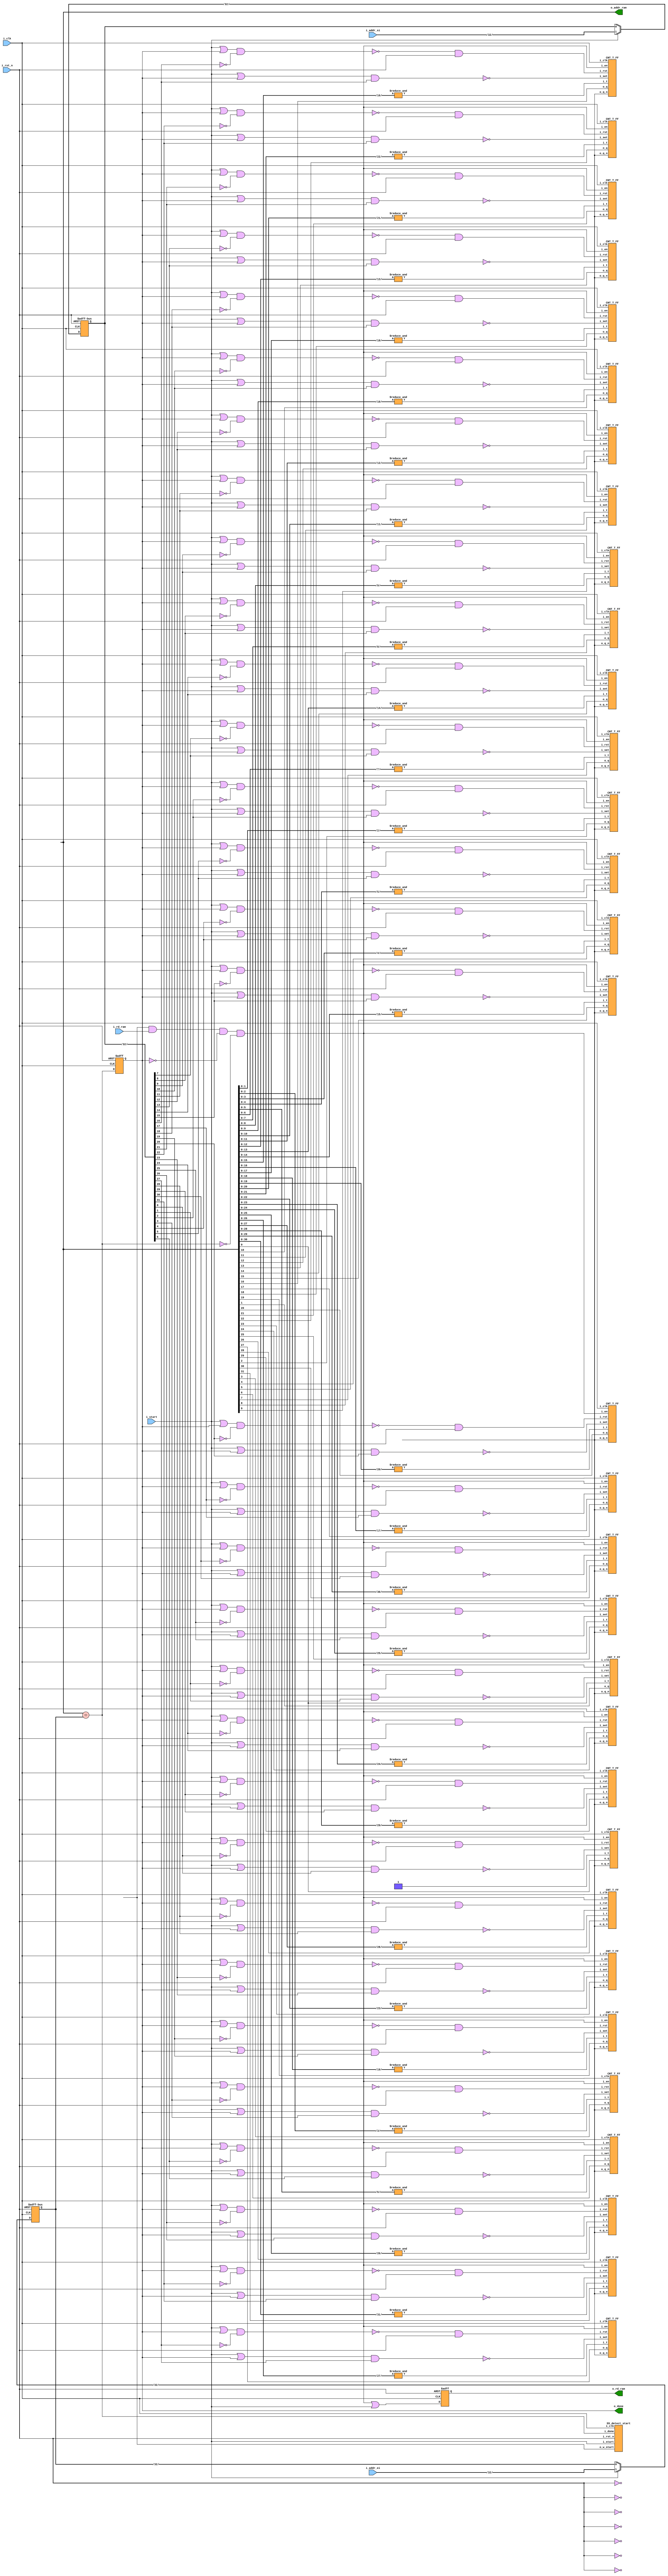
\includegraphics[width=.2\linewidth]{./../Version1/02_rtl/PA_CAL_MEAN/00_spec/PACS_control_address_diagram.png}
	\caption{Bộ điều khiển dữ liệu đọc với Memory Unit.}
\end{figure}

\begin{figure}[H]
	\centering
	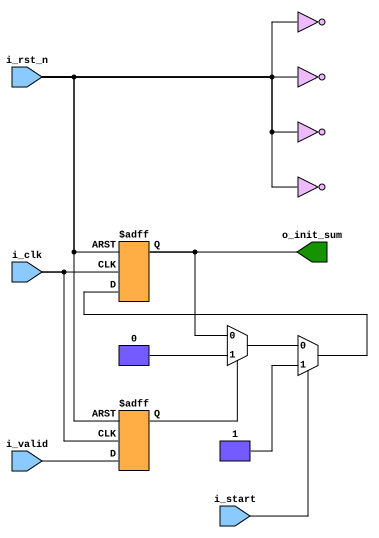
\includegraphics[width=.4\linewidth]{./../Version1/02_rtl/PA_CAL_MEAN/00_spec/PACS_detect_init_data.png}
	\caption{Bộ phát hiện tính hiệu bắt đầu.}
\end{figure}

\begin{figure}[H]
	\centering
	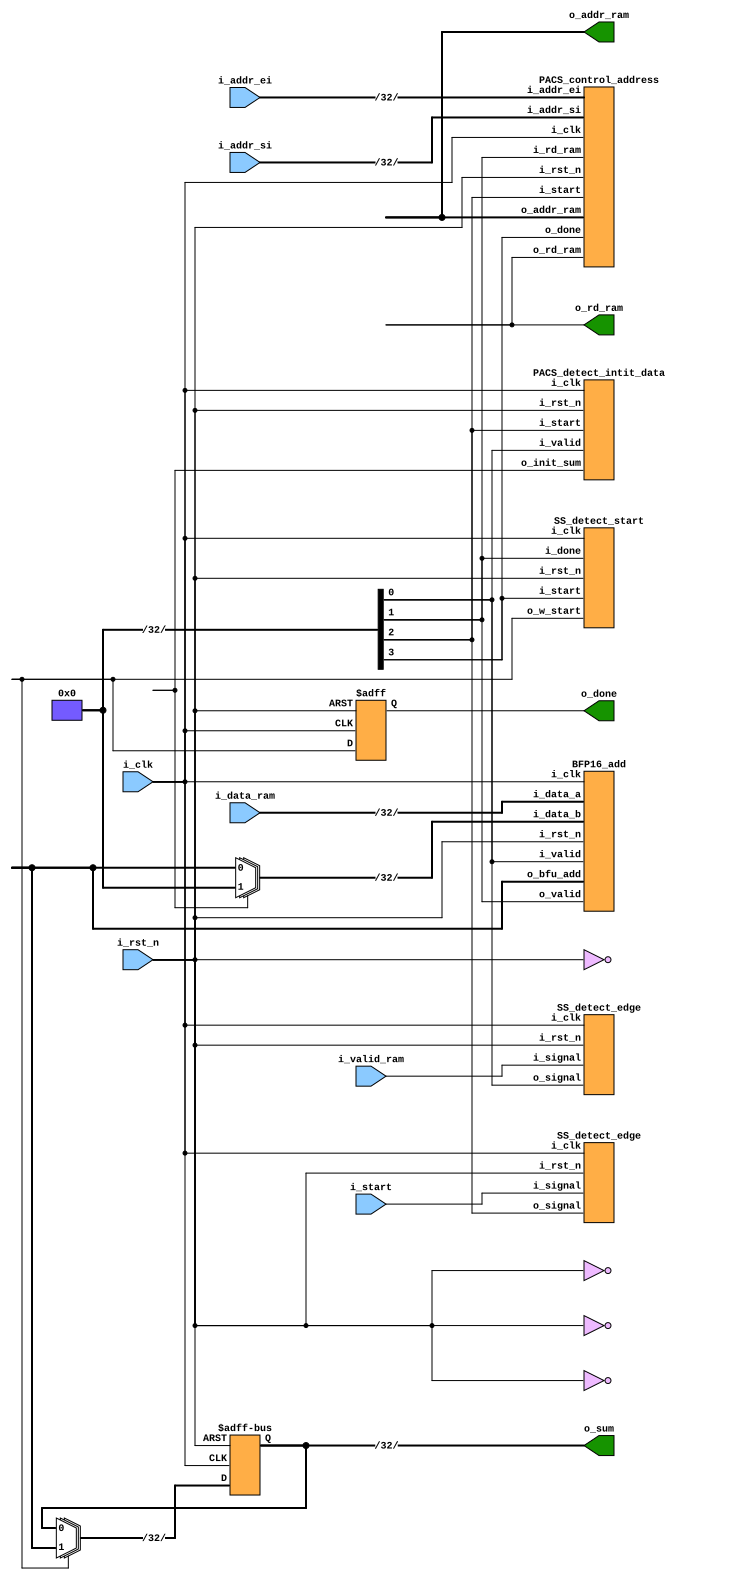
\includegraphics[width=.4\linewidth]{./../Version1/02_rtl/PA_CAL_MEAN/00_spec/PA_cal_sum_diagram.png}
	\caption{Bộ tính cộng số thực (BFP16\_add).}
\end{figure}

\subsubsection{Bộ tính chia số thực (FP32\_div)}

\begin{figure}[H]
	\centering
	\includegraphics[width=.5\linewidth]{./../Version1/02_rtl/PA_CAL_MEAN/BFP16_DIV/00_spec/FPU32_div_diagram.png}
	\caption{Bộ chia số thực.}
\end{figure}

\subsection{Bộ thực hiện partition lại mảng theo giá trị trung bình (PAMEM\_UNIT)}

\subsection{Bộ thực hiện đệ quy cho giải thuật (DI\_UNIT)}

\begin{figure}[H]
	\centering
	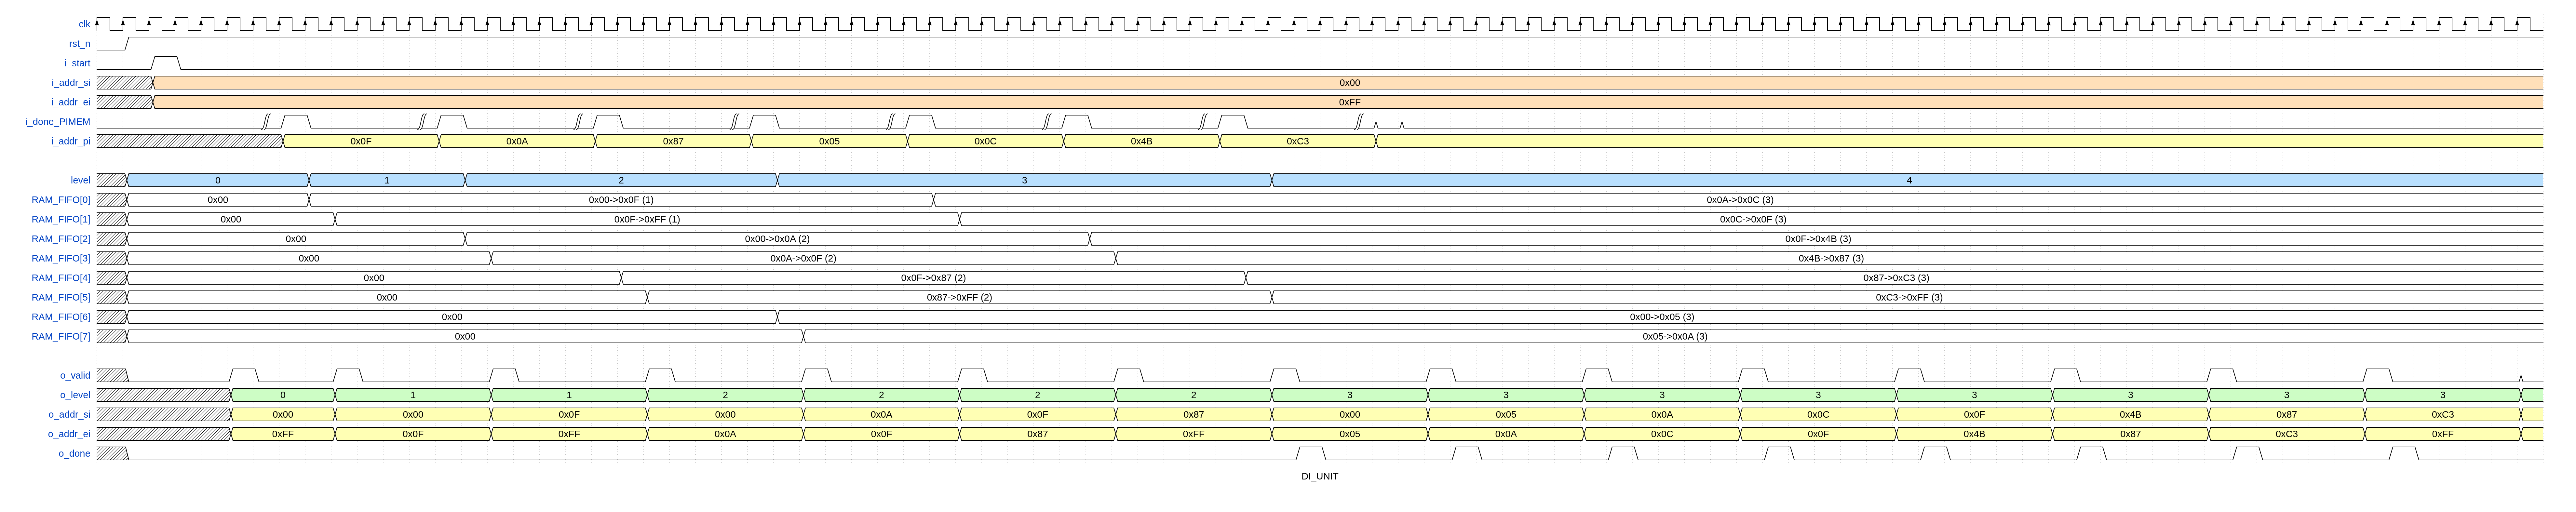
\includegraphics[width=\linewidth]{./../Version1/02_rtl/DI_UNIT/00_spec/WaveDrome_DI_unit.png}
\end{figure}
\include{./my-chapters/verification.tex}

\newpage
%\Myref{my-bib/ref}
%\section*{References}%
\addcontentsline{toc}{section}{References}%
\bibliographystyle{ieeetr}%
\bibliography{my-bib/ref}%
\end{document}


